% arara: pdflatex: { shell: yes }
% arara: biber
% arara: pdflatex: { shell: yes }
% arara: pdflatex: { shell: yes }

\documentclass[hidelinks, 12pt]{article}%

\usepackage{geometry} % useful for defining page geometries
\usepackage{hyperref} % used for creating hyperlinks in documents. Both to the web and within the document itself
\usepackage[tbtags]{amsmath} % for typesetting math (American Mathematical Society)
\usepackage{amsfonts} % fonts and mathematical symbols
\usepackage{amssymb} % more mathematical symbols
\usepackage[utf8]{inputenc} % how to treat the written file (as utf8)
\usepackage[T1]{fontenc} % the encoding for the output file T1 is the most common, includes accents and many other commonly needed/used characters
\usepackage[style=ieee,backend=biber]{biblatex} % for handling bibliographies
\usepackage{float} % added control over
\usepackage{graphicx} % tools for inclusion of graphics
\usepackage{booktabs} % adding commands to improve the look of tables
\usepackage{csvsimple} % simplify table creation by importing .csv files directly
\usepackage{siunitx} % consistent notation and correct formatting of units
\DeclareSIUnit{\torr}{Torr} % Custom unit definition
\usepackage{minted} % inclusion of code blocks with syntax highlighting and
\setminted{linenos, autogobble, fontsize=\footnotesize, breaklines=true} % set global options for minted environments
\usepackage{chemformula} % for writing chemical formulae

\addbibresource[location=local]{references.bib} % adding a bibliography

\begin{document}
    \begin{center}
        \vspace*{1cm}
        {\fontsize{300}{50}\selectfont {\bfseries Hello \LaTeX\\}}
        \vspace{3cm}
        {\LARGE An Introduction to the\\
            Typesetting Tool\\}
        \vspace{9cm}
    \end{center}
    \begin{raggedleft}
        {\Large Aaron English\\
            Ghassan Arnouk\\
            Date: \today\\}
    \end{raggedleft}
    \thispagestyle{empty}

    \clearpage
    \tableofcontents
    \clearpage
    \section{Motivation}
        \begin{itemize}
            \item High quality documents
            \item Automation
            \item Widely available and extraordinarily flexible
            \item Open-Source (and free)
            \item Enormous and extremely helpful user base
                \begin{itemize}
                    \item \href{https://www.overleaf.com/learn}{Overleaf guides}
                    \item \href{https://tex.stackexchange.com/}{TeX Stack Exchange}
                    \item \href{https://www.ctan.org/}{CTAN - Comprehensive TeX Archive Network}
                \end{itemize}
            \item Nearly unlimited skillcap - actual benefits to improving
        \end{itemize}


    \section{Base Packages}
        There are a few base packages that you should (almost) always import:
        \begin{enumerate}
            \item import
            \item geometry
            \item hyperref
            \item amsmath
            \item amsfonts
            \item amssymb
            \item inputenc
            \item fontenc
            \item biblatex
            \item float
            \item graphicx
        \end{enumerate}
        ...And a few that you'll typically include (and are used to prepare this document).
        \begin{enumerate}
            \item booktabs - Pretty professional tables
            \item csvsimple - Simplify table generation
            \item siunitx - Nice, clean, units
            \item minted - Beautiful blocks of highlighted code thanks to Pygments
            \item chemformula - Convenient chemical equation display
        \end{enumerate}

        \begin{listing}[H]
            \begin{minted}{tex}
                \usepackage{import}
                \usepackage{geometry}
                \usepackage{hyperref}
                \usepackage[tbtags]{amsmath}
                \usepackage{amsfonts}
                \usepackage{amssymb}
                \usepackage[utf8]{inputenc}
                \usepackage[T1]{fontenc}
                \usepackage[style=ieee,backend=biber]{biblatex}
                \usepackage{float}
                \usepackage{graphicx}
                \usepackage{booktabs}
                \usepackage{csvsimple}
                \usepackage{siunitx}
                \usepackage{minted}
                \usepackage{chemformula}
            \end{minted}
            \caption{Code to include packages in a \LaTeX document (as used in this document)}
            \label{lst:packages}
        \end{listing}

    \section{Sections...}
        \subsection{...and subsections...}
            \subsubsection{...and subsubsections...}

    \section{Equations}
        How about some equations?
        \begin{align}
            \delta & = - \frac{B^{2}}{180,000} + \frac{B}{173} + 0.5\nonumber      \\
                   & = - \frac{533^{2}}{180,000} + \frac{533}{173} + 0.5 \nonumber \\
                   & = 2.0 \nonumber
        \end{align}

        Or even a matrix
        \begin{equation*}
            A =
            \begin{bmatrix}
                -\alpha_f-\beta_1 & 2                 & \frac{1}{c} \\
                -4i               & \sqrt{5-\alpha_f} & -6          \\
                c                 & \beta_1           & 9 + i
            \end{bmatrix}
        \end{equation*}

        Calculus!
        \begin{align}
            \frac{\text{d}x}{\text{d}t} &= \sigma (y-x)\\
            \frac{\text{d}y}{\text{d}t} &= x(\rho -z)-y\\
            \frac{\text{d}z}{\text{d}t} &= xy-\beta z
        \end{align}
        An example with an integral, the Fourier Transform
        \begin{equation}
            \hat{f}\left(\xi\right) = \int_{-\infty}^{\infty}f\left(\xi\right)e^{2\pi ix\xi}\text{d}\xi
            \label{eqt:fourTrans}
        \end{equation}


    \clearpage
    \section{Figures}
        You can add lovely figures, and then reference them like this "As stated in Figure \ref{fig:test}".
        It's even a hyperlink! \textit{*click* *click*}

        \begin{figure}[H]
            \begin{centering}
                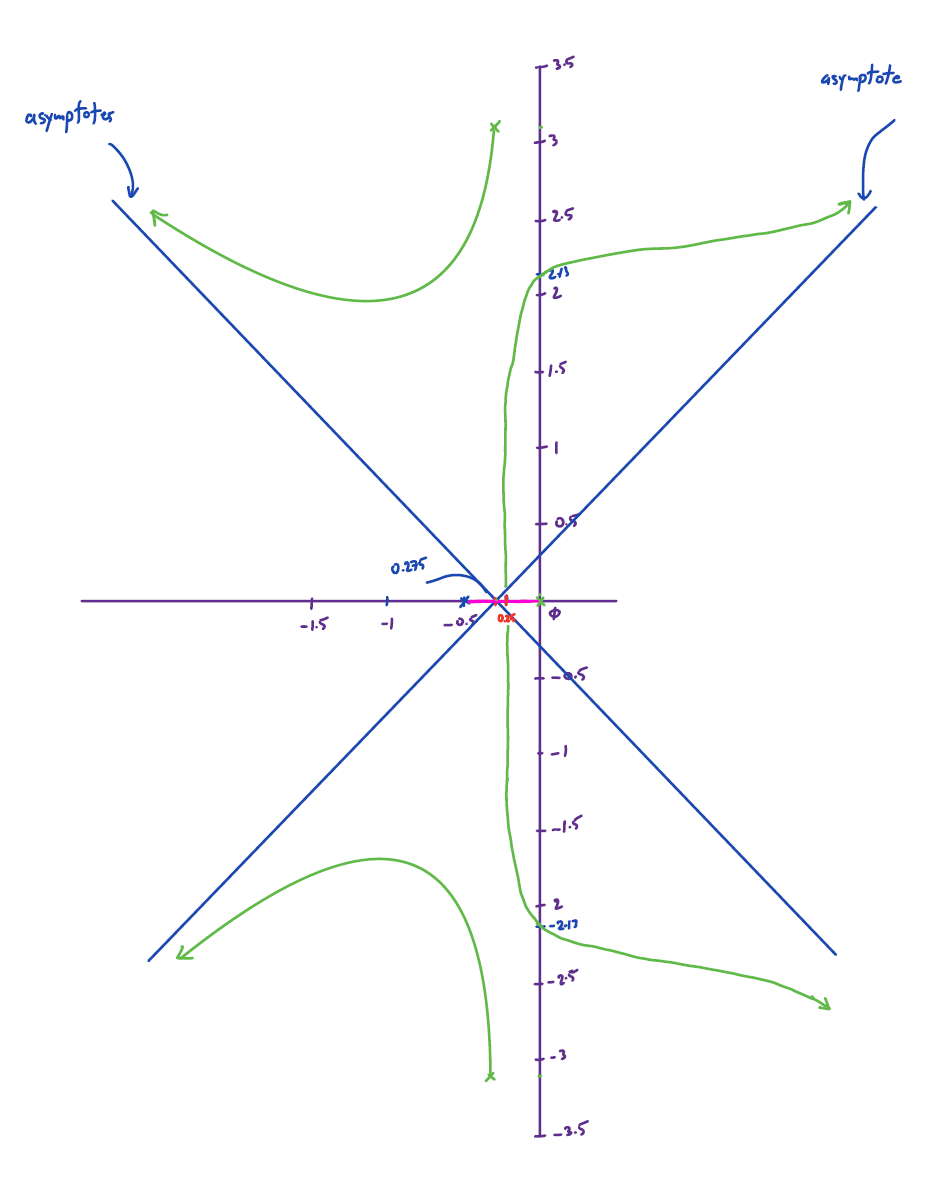
\includegraphics[width=0.5\textwidth]{images/rootLocus.png}
                \caption{A test figure}
                \label{fig:test}
            \end{centering}
        \end{figure}

    \section{Tables}
        What are tables like?
        Like this!
        \begin{table}[H]
            \centering
            \caption{Table of specified parameters and achieved values}
            \vspace{0.1cm}
                \csvreader[
                head to column names,
                tabular = cccc,
                table head = \toprule \bfseries Parameter & \bfseries Target & \bfseries Calculated & \bfseries Simulated \\\midrule,
                table foot = \bottomrule,
                ]{data/TargetsAndVals.csv}{}{\csvcoli & \csvcolii & \csvcoliii & \csvcoliv}
            \label{Table:Parameters}
        \end{table}

    \section{Additional Helpful Packages}
        \begin{itemize}
        \item siunitx
            I strongly recommend using the siunitx package for formatting all units.
            \\\si{\hertz}
            \\\SIrange{100}{200}{\nano\meter}
            \\\SI{100}{\kilo\gram}
            \\Convenient!

        \item minted
            \begin{listing}[H]
                \inputminted{python}{./demo.py}
                \caption{An example of a block of python included and highlighted with the package minted}
                \label{lst:pythonExample}
            \end{listing}

        \item chemformula
            A chemical (or nuclear) equation!
            \begin{equation}
                \ch{
                ^{2}H + ^{2}H -> ^{3}He + n^{0}
                }
                \label{eqt:nucEnerReleased}
            \end{equation}
            \end{itemize}


    \section{Bibliography}
        \subsection{Writing the .bib File}
            \begin{listing}[H]
                \begin{centering}
                    \begin{minted}{bibtex}
                        @incollection{ref:01,
                        author = {Berger, M.J. and Hubbell, J.H. and Seltzer, S.M. and Chang, J. and Coursey, J.S. and Sukumar, R. and Zucker, D.S. and Olsen, K.},
                        title = {XCOM: Photon Cross Sections Database},
                        publisher = {NIST, PLM, Radiation Physics Division},
                        year = {2010},
                        booktitle = {NIST Standard Reference Database 8 (XGAM)},
                        chapter = {Copper},
                        url = {https://physics.nist.gov/cgi-bin/Xcom/xcom3_1},
                        }
                    \end{minted}
                    \caption{Code for a bibliographic entry}
                    \label{lst:bibliography}
                \end{centering}
            \end{listing}
            While you may have to write a bib entry manually occasional, almost all journal websites offer .bib citations to copy and paste (or download).
            There are also a number of tools that simplify .bib generation:
            \begin{itemize}
                \item Lookup books by their ISBN and get a bibtex entry \href{https://lead.to/amazon/com/?key=+&si=all&op=bt&bn=&so=sa&ht=us}{lead.to}
                \item Browser extension to create bibtex entries from the current webpage (available for firefox and chrome)\href{https://github.com/Langenscheiss/bibitnow}{bibitnow}
                \item many others
            \end{itemize}
        \subsection{Using the References}
            Here I am making a statement that should be backed up with a reference placed right at the end. \cite{ref:01}
            Now it will show up in the bibliography and the reference above will link to it and be
            correctly numbered. For Free!

    \clearpage
    \printbibliography[heading=bibintoc]
\end{document}
